\section{Array}
Array adalah variabel jamak, yang mempunyai banyak elemen yang diacu dengan satu nama yang sama. Array (atau larik dalam bahasa indonesia) bukanlah tipe data dasar seperti integer atau boolen, Array adalah sebuah tipe data bentukan yang terdiri dari kumpulan tipe data lainnya. Menggunakan array akan memudahkan dalam membuat kelompok data, serta menghemat penulisan dan penggunaan variabel. berikut sebagai contoh
 \begin{lstlisting}
<?php
    $a = array("budi", 20, 58.5);
?>
\end{lstlisting}
Array dalam PHP juga merupakan tipe data, bukan sekedar variabel. Berikut merupakan jenis array dalam PHP:
\subsection{Array Berindeks}
Array berindeks adalah array yang diindeks berdasarkan nomor/angka. Indeks array pada umumnya dimulai dari angka 0. Anda bebas mendefinisikan indeks dengan nilai yang Anda tentukan.

\begin{table}[h]
\caption(Array Berindeks}
\centering
\begin{tabular}
\hline
\textbf{10}&\textbf{20}&\textbf{30}&\textbf{40}&\textbf{50}\\
\hline

\begin{lstlisting}
 $a[0]
\end{lstlisting}  & 

\begin{lstlisting}
 $a[1]
\end{lstlisting} &

\begin{lstlisting}
 $a[2]
\end{lstlisting} &

\begin{lstlisting}
 $a[3]
\end{lstlisting} &

\begin{lstlisting}
 $a[4]
\end{lstlisting}\\
\hline
\end{tabular}
\label{tabel : Array Berindeks}
\end{table}


Contoh diatas menunjukan array dengan 5 buah elemen. Elemen pertama ($a[0]) bernilai 10, elemen
kedua ($a[1]) bernilai 20, dan seterusnya. Dalam array berindeks, antara kunci (indeks) dan nilai tidak
memiliki keterkaitan.

\subsection{Array Asosiatif}
Array asosiatif adalah array yang diindeks berdasarkan nama tertentu. Letak perbedaan antara array berindeks dan array asosiatif adalah hanya terletak pada penamaan indeksnya saja.
\begin{table}[h]
\caption(Array Asosiatif}
\centering
\begin{tabular}{|c|c|c|c|c|}
\hline
\textbf{10}&\textbf{20}&\textbf{30}&\textbf{40}&\textbf{50}\\
\hline

\begin{lstlisting}
 $a["satu"]
\end{lstlisting}  & 

\begin{lstlisting}
 $a["dua"]
\end{lstlisting} &

\begin{lstlisting}
 $a["tiga"]
\end{lstlisting} &

\begin{lstlisting}
 $a["empat"]
\end{lstlisting} &

\begin{lstlisting}
 $a["lima"]
\end{lstlisting}\\
\hline
\end{tabular}
\label{tabel : Array Asosiatif}
\end{table}

Array diindeks berdasarkan nama, bukan berdasarkan nomor. Pada contoh diatas indeks array bertipe string. Pada umumnya array asosiatif digunakan untuk merepresentasikan sesuatu yang kunci dan nilainya memiliki keterkaitan, misalnya sebagai berikut.

\begin{lstlisting}
 <?php
  $kota = array("jkt" => "jakarta", "bdg" => "bandung", "sby" => "surabaya");
 ?>
\end{lstlisting}  


\section{Membuat Array}
Array dapat dibuat melalui dua cara, yaitu dengan menggunakan fungsi array() atau dengan membuat elemen-elemen array dan mengisikan nilai-nilai ke dalam elemen-elemen tersebut secara langsung.
Berikut ini contoh pembuatan array dengan menggunakan fungsi array().

\item{Untuk Array Berindeks}
\begin{lstlisting}
<?php
 $matakuliah = array ("pemograman web", "database", "keamanan jaringan",
 "sistem informasi", "rekayasa perangkat lunak");
 ?>
\end{lstlisting}

\item{Untuk Array Asosiatif}
\begin{lstlisting}
<?php
$detailmk = array ("kode" => "TKB5218", "nama" => "pemograman web 2", "sks" => 2);
?>
\end{lstlisting}

Berikut ini contoh pembuatan array dengan cara langsung membuat variabel array dan mengisikan nilai ke dalamnya.

\item{Untuk array berindeks}
\begin{lstlisting}
<?php 
$matakuliah[0] = "pemograman web"; 
$matakuliah[1] = "database"; 
$matakuliah[2] = "keamanan jaringan"; 
$matakuliah[3] = "sistem informasi"; 
$matakuliah[4] = "rekayasa perangkat lunak"; 
?>
\end{lstlisting}

\item{Untuk array asosiatif}
\begin{lstlisting}
<?php 
$detailmk["kode"] = "TKB5218"; 
$detailmk["nama"] = "pemograman web 2"; 
$detailmk["sks"] = 2; 
?>
\end{lstlisting}

\subsection{File & Direktori}
Dalam management file dan direktori, PHP menyediakan lebih 70 fungsi. Beberapa fungsi utama yang berhubungan dengan management file (create, write, append, dan delete), antara lain : Membuka dan membuat file.
\begin{lstlisting}
fopen ($namafile, $mode);
\end{lstlisting}
Keterangan :
namafile merupakan nama file yang akan dibuat, sedangkan mode merupakan mode akses file. Contoh:
\begin{lstlisting}
<?php
$namafile = "data.txt";
$handle = fopen ($namafile, "mode");
if (!handle) {
	echo "<b>File yang ada buat belum ada</b>";
} else {
	echo "<b>File telah berhasil dibuka</b>";
}
fclose($handle);
?>
\end{lstlisting}


\subsection{Pemrograman Berorientasi Objek Dalam PHP }
PHP pada awalnya hanya sekumpulan script sederhana. Dalam perkembangannya, dapat ditambahkan berbagai fitur pemrograman berorientasi objek. Hal ini dimulai sejak PHP 4. Dengan lahirnya PHP 5, fitur-fitur pemrograman berorientasi objek semakin mantap dan semakin cepat. Dengan PHP 7, script yang menggunakan konsep object-oriented akan lebih cepat dan lebih efisien.
\par
Pemrograman berorientasi objek atau object-oriented programming (OOP) merupakan suatu inovasi dalam pemrograman yang menggunakan object dan class. Saat ini konsep OOP sudah semakin berkembang. Hampir setiap perguruan tinggi di dunia mengajarkan konsep OOP ini pada mahasiswanya. Pemrograman yang banyak dipakai dalam penerapan konsep OOP adalah Java dan C++. OOP bukanlah sekedar cara penulisan sintaks program yang berbeda, namun dapat lebih dari itu, OOP merupakan cara pandang dalam menganalisa sistem dan permasalahan pemrograman. Dalam OOP, setiap bagian dari program adalah object. Sebuah object mewakili suatu bagian program yang akan diselesaikan. Beberapa konsep OOP dasar, antara lain :
\begin{enumerate}
\item Encapsulation (Class dan Object)
\item Inheritance (Penurunan sifat)
\item Polymorphisme
\end{enumerate}
\par
PHP khususnya PHP 7 sudah mendukung beberapa konsep OOP. Akan tetapi PHP 7 tidak mendukung konsep Multiple-inheritance dan polymorphisme.

\subsection{ Object Dan Class}
Bagian dasar dari program yang berorientasi objek adalah objects. Secara tidak langsung  kita dapat memahami mengenai object ini. Sebagai contoh, sebuah mobil adalah objek. Sebuah mobil mempunyai properties atau bagian-bagian di dalamnya, seperti warna, mesin, roda, pintu dsb. Sebuah mobil juga dapat melakukan sesuatu, seperti mengisi bensin, menyalakan mesin, berjalan, mengerem dsb. 
\par
Biasanya object adalah sebuah kata benda. Orang adalah object. Demikian juga mobil, pohon, bunga, komputer, TV, buku dsb. Namun, object tidak selamanya sebuah objek fisik. Bisa saja sebuah benda abstrak, seperti account bank, sebuah file di komputer, database, pesan email, acara TV, dsb. 
Class merupakan penjelasan atau deskripsi dari object. Di dalam class, terdapat penjelasan tentang suatu object termasuk properties yang dimilikinya dan kelakuan atau method yang bisa dilakukan oleh object. Sebagai contoh, class Orang. Class Orang tentu setidaknya memiliki beberapa bagian seperti tangan, kaki, mata, telinga dsb. Class Orang juga setidaknya harus bisa jalan, bisa loncat, bisa lari, bisa melihat, bisa bicara dsb. 
\par
Salah satu keuntungan program didefinisikan dengan konsep OOP adalah adanya pengkapsulan (encapsulation) program dalam class dan object, dimana sang programmer yang menggunakan class tidak perlu mengetahui isi dan jalannya class secara detail, hanya perlu tahu bagaimana cara menggunakannya. Sama halnya dengan sebuah mobil misalnya. Seorang pemilik mobil tentunya tidak perlu mengetahui bagian-bagian mobil secara menyeluruh. Dia tidak perlu mengetahui bagaimana mesin mobil melakukan pembakaran dan bagaimana mesin mobil bisa menggerakkan roda, dsb. Dia hanya perlu tahu bagaimana cara menjalankan mobil, bagaimana menghentikan mobil, dan fungsi mobil lainnya. 

\subsection{Properties Dan Method}
Setiap class dapat memiliki properties yang kadang disebut juga attributes. Properties sebuah mobil misalnya warna, ukuran, harga dsb. Di dalam class, properties dapat dinyatakan dengan sebuah variabel. Misalnya warna, harga, dsb. Method merupakan sesuatu yang bisa dilakukan oleh object. Method dalam PHP sama halnya dengan sebuah fungsi. Method yang mungkin mempunyai
sebuah mobil misalnya, method untuk menghidupkan mobil, menjalankan mobil, menghentikan mobil, dsb. Penamaan properties dan method memiliki sejumlah aturan yang sama dengan penamaan sebuah variabel atau fungsi. Akan tetapi berdasarkan kesepakatan
(convention), penamaan properties dan method harus menggunakan camel Caps, dimana tiap kata diawali dengan huruf besar kecuali kata pertama, setiap kata digabung tanpa spasi atau under-score.
\par
Mendefinisikan Class bentuk umum untuk mendefinisikan sebuah class contohnya sebagai berikut:
\begin{lstlisting}
class namaClass
{
Deklarasikan dan definisikan properties di sini
Definisikan semua method di sini
} 
\end{lstlisting}

Penamaan namaClass pada dasarnya sama dengan penamaan variabel. Penamaannya bebas, boleh apa saja, kecuali stdClass. PHP sudah menggunakan nama stdClass sebagai nama class built-in. Isi tubuh class terletak di antara tanda kurung kurawal buka  dan kurawal tutup. Di tubuh class terdapat pendefinisian properties (variabel) dan method-method class. 


\subsection{Mengakses Elemen Array}
Setelah array dibuat, langkah selanjutnya adalah mengakses nilai-nilai yang terkandung di dalamnya.
Cara mengakses elemen array sangatlah sederhana. Karena elemen array berupa nilai, maka kita dapat
memperlakukannya seperti layaknya variabel.
Kita dapat menempatkan nilai yang diakses ke dalam suatu variabel atau dapat juga diproses secara
langsung baik dalam perhitungan maupun ditampilkan langsung.
Berikut ini adalah contoh mengakses nilai array ke dalam suatu variabel.
\lstinputlisting[firstline=1, lastline=9]{src/array.php}

Berikut ini adalah contoh mengakses elemen array secara langsung
\lstinputlisting[firstline=1, lastline=23]{src/akses_array.php}

\subsection{Fungsi-fungsi yang berhubungan dengan array}
Berikut ini beberapa fungsi yang dapat digunakan pada variabel bertipe array.
\begin{figure}[!htbp]
 \centering
 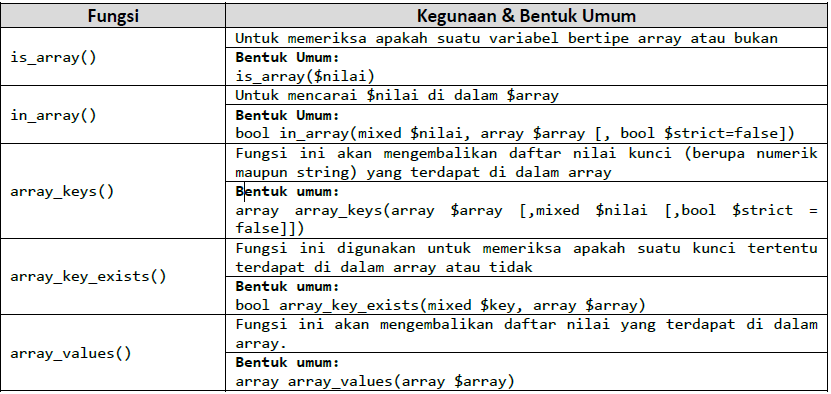
\includegraphics[width=.90\textwidth]{figures/fungsi_array.png}
\end{figure}

\begin{figure}[!htbp]
 \centering
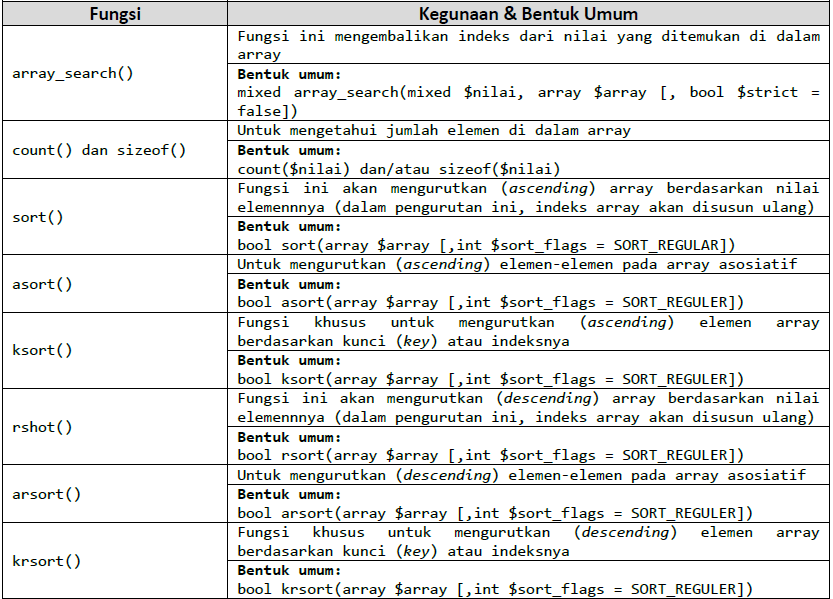
\includegraphics[width=.90\textwidth]{figures/fungsi_array2.png}
 \caption{Fungsi-fungsi yang berhubungan dengan array}\label{fig:inputchapter}
\end{figure}

